% Created 2022-06-21 Tue 23:00
% Intended LaTeX compiler: pdflatex
\documentclass[11pt]{article}
\usepackage[utf8]{inputenc}
\usepackage[T1]{fontenc}
\usepackage{graphicx}
\usepackage{longtable}
\usepackage{wrapfig}
\usepackage{rotating}
\usepackage[normalem]{ulem}
\usepackage{amsmath}
\usepackage{amssymb}
\usepackage{capt-of}
\usepackage{hyperref}
\usepackage{cleveref}
\usepackage{subfig}
\usepackage[letterpaper, vmargin=1in, lmargin=0.75in, rmargin=3in, marginparwidth=2.25in, marginparsep=0.25in]{geometry}
\usepackage{fancyhdr}
\pagestyle{fancy}
\usepackage{amssymb}
\usepackage{soul}
\usepackage{color}
\usepackage[citestyle=authoryear,bibstyle=authoryear, hyperref=true,backref=true,maxcitenames=3,url=true,backend=biber,natbib=true] {biblatex}
\addbibresource{export/bibs.bib}
\fancyhead[CO,CE]{\textbf{[Align-BDD]}}
\fancyhead[LO,LE]{A.B.}
\fancyhead[RO,RE]{Appl.: j-UFLP, note 2.}
\usepackage{marginnote}
\usepackage{tikz}
\usepackage{algorithm}
\usepackage{algpseudocode}
\renewcommand{\algorithmicrequire}{\textbf{Input:}}
\renewcommand{\algorithmicensure}{\textbf{Output:}}
\renewcommand{\Comment}[1]{\textit{\ // #1}}
\newcommand{\return}[1]{\textbf{return} #1}
\newcommand{\hi}[1]{\texttt{HI(#1)}}
\newcommand{\lo}[1]{\texttt{LO(#1)}}

% describing environments
\usepackage{amsthm}
\newtheorem{proposition}{Proposition}
\author{Alexey Bochkarev}
\date{\today}
\title{Align-BDD: encoding j-UFLP with BDDs.}
\hypersetup{
 pdfauthor={Alexey Bochkarev},
 pdftitle={Align-BDD: encoding j-UFLP with BDDs.},
 pdfkeywords={},
 pdfsubject={},
 pdfcreator={Emacs 27.1 (Org mode 9.5.2)}, 
 pdflang={English}}
\begin{document}

\maketitle

\section{Summary}
\label{sec:orgc3a554e}
\marginnote{
\textbf{Context:} We have been constructing BDDs for the CPP using auxiliary, smaller MIPs. It is faster
than a naive MIP, but seems to allow very limited sensitivity analsysis. Moreover, it turned out
it is quite often slower than CPP MIP. Therefore, we decided to revert to full BDDs (where one layer
= one decision variable, $x_i$) that would not require solving any auxiliary MIPs. This required a better way
to construct BDDs for UFLP, so I think I have found one.}[-6ex]
In this note I discuss a new way to create BDDs for the uncapacitated facility
location poroblem (UFLP) that yields more compact diagrams, and another
numerical experiment with joint-UFLP (j-UFLP) comparing the three approaches:
\begin{itemize}
\item a naive MIP,
\item a CPP MIP,
\item a shortest-path CPP.
\end{itemize}

The results are perhaps more promising than the ones we had before, but I would
  like to discuss and invent yet another special class of j-UFLP instances that
  would allow to highlight the numerical benefits of the computational pipeline
  we propose. Let us see if we can achieve this using this new understanding of
  how the diagrams are actually built for UFLP.

\section{Encoding UFLP with BDDs}
\label{sec:org0eb0cfa}
\subsection{Creating a BDD for a given order of variables}
\label{sec:org8e50c41}
Let us start with a BDD construction for a single UFLP instance, which is
equivalent to the following MIP: \marginnote{This is the same
formulation as before, for a single UFLP.}
\begin{subequations}\label{eq:UFLP}
\begin{align}
  \min & \sum_{i=1}^N \Big(c_i x_i + f_i(a_i)\Big)&\\
    \textrm{s.t. } & a_i = \sum_{j\in S_i} x_i& \textrm{ for all } i=1,\ldots, N,\\
    & x_i\in\{0,1\} & \textrm{ for all } i=1,\ldots,N,\\
\end{align}
\end{subequations}
where \(S_i\) is a list of points adjacent to \textcircled{$i$} (including itself,
by assumption). We seek to build a BDD where every layer would represent a
single facility location decision, \(x_i\). Technically, each node of the BDD will
be associated with a \emph{state} \(\sigma = (s_1, \ldots, s_N)\), where
\(s_i\in\{1,0,*\}\) represents whether a facility has been located (\(s_i=1\)) at
\textcircled{$i$} or not (\(s_i=0\)). The third value, \(s_i=*\), indicates that the
decision on point \textcircled{$i$} does not affect costs, and hence, does not
matter at this moment of the BDD construction, or simply not yet known.
\marginnote{We do not impose any hard constraints, so, nothing can
affect \textit{feasibility}, only costs are relevant.}[-2em] Each node state
is unique within the respective layer. As we incorporate more decisions and the
corresponding costs to the diagram, some previous decisions become irrelevant
and the layer width can both increase or decrease. Let us try to find a good
order of decisions to keep the BDD size small.

There are two key observations relevant to the BDD construction. First, we can
\textbf{incorporate costs} associated with point \(i\), \(c_i x_i + f_i(a_i)\), as soon as
we incorporate all decisions \(x_j\in S_i\). For the situation depicted in Figure
\ref{fig:Ns}, we can calculate costs associated with \textcircled{$i$} only when
we incorporate all decisions regarding the gray points and \textcircled{$i$}
itself. After that we can derive \(x_i\) and \(a_i\) (to compute \(f_i(a_i)\) from
each BDD node state as discussed above. However, incorporating all points from
\(S_i\) is not enough to discard the decision regarding point \textcircled{$i$}
(marking it \(*\) in all further node states). For example, the cost associated
with point \textcircled{$j$} in Figure \ref{fig:Ns} depends on the decisions
regarding points \textcircled{$i$}, \textcircled{$j$}, and all the points shaded
with dark color. Therefore, we will have to keep the decision on
\textcircled{$i$} in the state until we incorporate all the points depicted in
the figure (assuming no other points are present). This is the second key
observation regarding the BDD construction:

Any point \textcircled{$i$} can be marked \textbf{``irrelevant''} in the node state
(\(s_i\) set to \(*\)) as soon as we have incorporated the decisions regarding all
points \(j\in S^*_i = \{j:~d(i,j)\leq 2\}\) into the diagram.

These two observations both yield an algorithm to construct the diagram given an
order of points to incorporate, and suggest a way to find a good order of
decisions. Let us start with the former.

Algorithm \ref{alg:UFLPDD} constructs the diagram encoding problem \eqref{eq:UFLP},
assuming pre-defined order of variables \(O\). For each point \textcircled{$i$},
we sustain two values. First, its \emph{cost uncertainty} \(Q_i\) is the number of
points we would need to incorporate into the diagram to be able to calculate the
cost associated with \textcircled{$i$}. Second, its \emph{value} \(V_i\) is the number
of points which costs depend on the decision on point \textcircled{$i$}. Every
time we incorporate new point \textcircled{$i$} into the diagram, we decrement
\(Q_j\) for all points from its neighborhood \(S_i\). After this step we can
calculate costs associated with all points \(j\) such that \(Q_j=0\). Further, each
time we calculate cost for some point \(j\) we can decrement \(V_k\) for all points
\(k\) from its neighborhood \(S_i\). Every time node value for some node \(V_k\) drops
to zero, we mark it as ``irrelevant'' by setting the corresponding state marker
to \(*\).

\begin{algorithm}
\scriptsize
\caption{create-UFLP-BDD}\label{alg:UFLPDD}
\begin{algorithmic}[1]
  \Require{Graph $G$, given by $S_i, i=1,\ldots, N$;
   costs $f_i(\cdot), c_i$ for $i=1,\ldots, N$; points order $O$.}
  \Ensure{BDD encoding the problem.}
  \State $Q_j \gets |S_j|$ for all $j=1,\ldots,N$ \Comment{Costs ``uncertainty'' for each node}
  \State $V_j \gets |S^*_j|$ for all $j=1,\ldots,N$ \Comment{Node ``value''.} 
  \State $\texttt{next-layer} \gets \{(*, \ldots, *)\}$ \Comment{Root node only.}
  \State $k \gets 1$ \Comment{Current layer number.}
  \While{$k<N$}
    \State $i \gets Q_k$ \Comment{The next point being incorporated into the diagram.}
    \State $P \gets \varnothing$ \Comment{Set of points to calculate costs for.}
    \State \textbf{decrement} $Q_j$ for all $j\in S_i$
    \State $P \gets P\cup \{j:~Q_j = 0,~j\in S_i\}$
    \State \textbf{decrement} $V_j$ for all $j\in \cup_{t\in P} S_t$
    \State $\texttt{current-layer} \gets \textbf{copy}(\texttt{next-layer})$
    \If{$k=N$}
      \State $\texttt{next-layer} \gets \{ (*, \ldots, *) \}$ \Comment{True terminal.}
    \Else
      \State $\texttt{next-layer} \gets \varnothing$.
    \EndIf
    \For{$\sigma=(\sigma_1, \ldots, \sigma_N) \in \texttt{current-layer}$}
      \State set \texttt{next-state}: $s_k \gets *$ if $V_k=0$, and $\sigma_k$ otherwise for $k=1,\ldots, N$.
      \If{$\texttt{next-state}\notin\texttt{next-layer}$}
        \State \textbf{create} node \texttt{next-state} in \texttt{next-layer}
      \EndIf
      \State calculate $a_j \gets \sum_{k\in S_j} s_k$ for all $j\in P$
      \State calculate arc cost $C \gets \sum_{j\in P} \Big(c_j s_j + f_j(a_j)\Big)$
      \State add arc \lo{$\sigma$} $\gets \texttt{next-state}$ (with cost $C$)
      \State update \texttt{next-state}: $s_i \gets 1$ if $V_i\neq 0$.
      \If{$\texttt{next-state}\notin\texttt{next-layer}$}
        \State \textbf{create} node \texttt{next-state} in \texttt{next-layer}
      \EndIf
      \State recalculate $a_j \gets \sum_{k\in S_j} s_k$ for all $j\in P$
      \State recalculate arc cost $C \gets \sum_{j\in P} \Big(c_j s_j + f_j(a_j)\Big)$
      \State add arc \hi{$\sigma$} $\gets \texttt{next-state}$ (with cost $C$)
    \EndFor
    \State $k\gets k+1$
  \EndWhile
\end{algorithmic}
\end{algorithm}

  \begin{figure}%
    \centering
    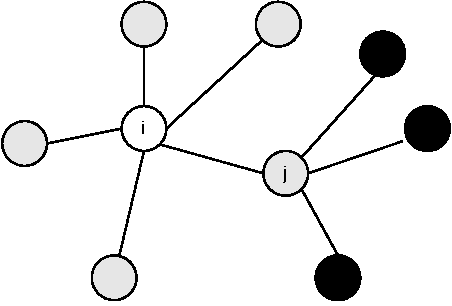
\includegraphics[width=0.7\textwidth]{./img/Ns.pdf}%
    \caption{Several points of the original graph.}\label{fig:Ns}%
\end{figure}

I think we can claim that given the order, this algorithm gives us the smallest
possible diagram:

\begin{proposition}
Given the target order of points, Algorithm \ref{alg:UFLPDD} produces the smallest
possible diagram that is valid for all cost parameters \(c_i\) and \(f_i(\cdot)\).
\marginnote{I need this \underline{valid for all costs} part: imagine
all the costs are just zero. Then, I can encode it as a BDD of width one.
Like, whatever I do, I'll have zero costs. That would not capture the
graph structure and would seriously restrict my sensitivity analsysis.}[-4em]
\label{prop:bestDD}
\end{proposition}
\subsection{Finding a good order of variables.}
\label{sec:orgd1ea1a1}
The procedure we have just introduced provides some insight into the size of the
resulting diagram. Assuming the size (width) of the current, $k$-th
layer is \(W_k\). Then, width of the next layer will be:
\[ W_{k+1} = W_k \times 2^{1 - F_k} = 2^{k - \sum_{j=1}^k F_j, \]
where \(F_j\) is the number of points marked irrelevant after step \(j\) of
Algorithm \ref{alg:UFLPDD}. Therefore, the logarithm of width will look like the
one presented in Figure \ref{fig:LW}. The top (red) line represents steps \(y=k\),
the bottom (blue) one represents cumulative number of nodes marked irrelevant.

\begin{figure}[h!]
\centering
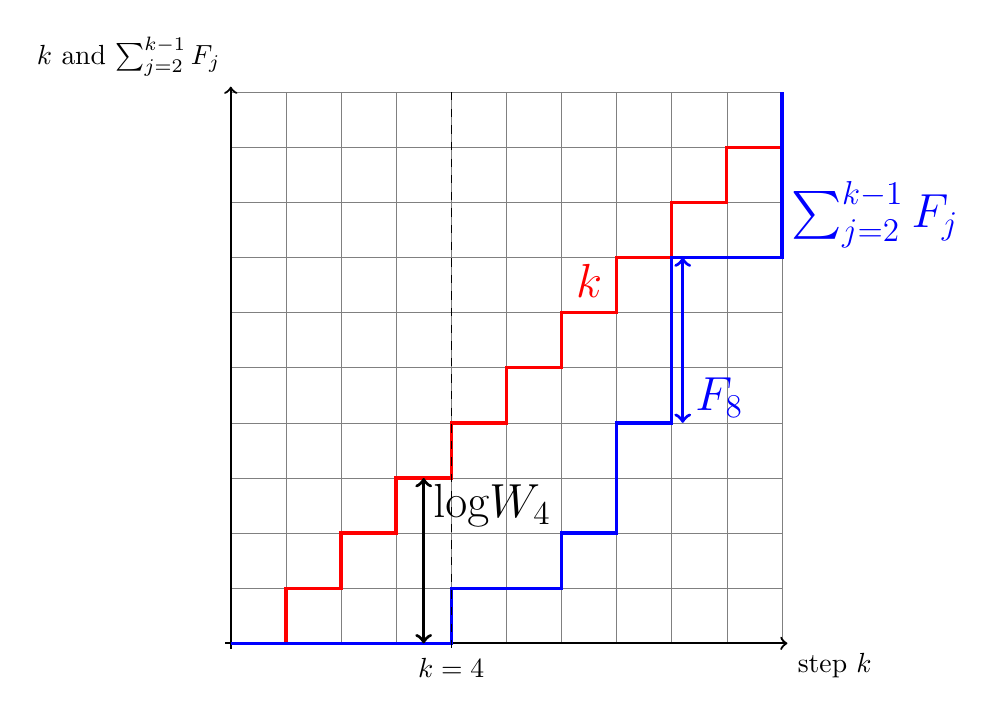
\begin{tikzpicture}[scale=0.7]
  \draw[step=1cm, very thin, gray] (0,0) grid (10,10); 
  \draw[thick, ->] (-0.1, 0) -- (10.1, 0) node[anchor=north west] {step $k$};
  \draw[thick, ->] (0, -0.1) -- (0, 10.1) node[anchor=south east] {$k$ and $\sum_{j=2}^{k-1}F_j$};
  \draw[very thick, red] (0,0) -- (1,0) -- (1,1) -- (2,1) -- (2,2) -- (3,2) -- (3,3) -- (4,3) -- (4,4) -- (5,4) -- (5,5) -- (6,5) -- (6,6) -- (7,6) -- (7,7) -- (8,7) -- (8,8) -- (9,8) -- (9,9) -- (10,9) -- (10,10);
  \draw (6.5,6.1) node[anchor=south]{\color{red} \LARGE $k$};
  \draw[blue, very thick, <->] (8.2,4) -- (8.2, 7);
  \draw (8.25, 5) node[anchor=north west] {\color{blue} \LARGE $F_8$};
  \draw (10, 7) node[anchor=south west] {\color{blue} \LARGE $\sum_{j=2}^{k-1}F_j$};
  \draw[very thick, blue] (0,0) -- (4,0) -- (4,1) -- (6,1) -- (6,2) -- (7,2) -- (7, 4) -- (8,4) -- (8,7) -- (10,7) -- (10,10);
  \draw[dashed] (4, 10) -- (4, -0.1) node[anchor=north] {$k=4$};
  \draw[very thick, <->] (3.5,0) -- (3.5,3);
  \draw (3.5,2.5) node[anchor=west] {\LARGE $\textrm{log}W_4$};
\end{tikzpicture}
\caption{An illustration for the layer width.}\label{fig:LW}
\end{figure}

This representation suggests a simple greedy algorithm, where at each
step we would try to complete the smallest set \(S^*_j\) (given the already taken
decisions). We illustrate it with Example \ref{ex:greedy}.

\begin{example}\label{ex:greedy}
Consider a graph depicted in Figure \ref{fig:ex-greedy}. We summarize the steps we
take in Table \ref{tab:greedy}. Rows represents distance-two-neighborhoods of
respective points. When we incorporate a point (add it to the BDD), we remove it
from further consideration by crossing it out from all the rows of the third
column (\(S^*_i\)) of the table. We keep track of the number of points left in
each subset in the right-most five columns of the table. \marginnote{For
example, when we incorporate points 1,2,3, and 4 into the BDD, we cross them out
from all the rows of that column and update the sizes of the subsets that are
left. For example, for subset \textcircled{3} (row 3) we had {1,2,3,4,5,6}.
After crossing out {1,2,3,4} we are left with {5,6}, which gives size 2 in
column $k=5$ (after step five).}[-3em]. The algorithm runs as follows:
\begin{itemize}
\item The smallest \(S^*_i\) corresponds to point 11 (with the single element, 11).
Therefore, we add point 11 and mark it irrelevant immediately.
\item The next candidate subset is \(S^*_1\) (of the smallest size 4, ignoring point
11 now). Hence we add points 1,2,3, and 4, and mark \textcircled{1} irrelevant.
\item We update the residual sizes of the length-2 neighborhoods (without elements
1,2,3,4, in addition to 11) in column \(k=5\) and observe that \textcircled{3}
can be marked irrelevant as well (points 1,2,3, and 4 are already added).
\item The next candidate subset to complete (corresponding to a smallest number in column
\(k=5\)) is \textcircled{$2$}. We add points 5 and 6, marking
\textcircled{$2$} as irrelevant.
\item The next candidate subset corresponds to a smallest number in column \(k=8\).
This would be the ones corresponding to \textcircled{4}, \textcircled{5}, or
\textcircled{6}. The first one is \textcircled{4}, \marginnote{We always
  pick the first subset, as we keep the them in a min-heap, keyed by the current
  size and breaking ties with the subset number.}[-5em] so we proceed with incorporating
points 7 and 10 into the diagram and marking \textcircled{4} as irrelevant.
\item The next candidates correspond to smallest numbers in column \(k=11\), which are
rows 5 or 6. Either way incorporate \textcircled{8} and mark both 5 and 6 as
irrelevant. Updated residual length-2 neighborhoods are presented in column
\(k=12\).
\item Finally, we add the last point, \textcircled{9} and mark 7, 8, 9, and 10 as
irrelevant, concluding the search for the best order.
\end{itemize}

This procedure results in the following solution: 11 | 1,2,3,4 | 5,6 | 7, 10 |
8 | 9  Here the points between the bars can be re-arranged at no
additional cost in terms of the BDD size. The corresponding layer width
diagram (similar to Figure \ref{fig:LW}) is presented in Figure \ref{fig:LW-ex}.

\begin{figure}[h!]
\centering
\begin{tikzpicture}[scale=0.7]
  \draw[step=1cm, very thin, gray] (0,0) grid (11,11); 
  \draw[thick, ->] (-0.1, 0) -- (11.1, 0) node[anchor=south west] {step $k$};
  \draw[thick, ->] (0, -0.1) -- (0, 11.1) node[anchor=south east] {$k$ and $\sum_{j=2}^{k-1}F_j$};
  \draw[very thick, red] (0,0) -- (1,0) -- (1,1) -- (2,1) -- (2,2) -- (3,2) -- (3,3) -- (4,3) -- (4,4) -- (5,4) -- (5,5) -- (6,5) -- (6,6) -- (7,6) -- (7,7) -- (8,7) -- (8,8) -- (9,8) -- (9,9) -- (10,9) -- (10,10) -- (11,10) -- (11,11);
  \draw (6.5,6.1) node[anchor=south]{\color{red} \LARGE $k$};
  \draw (11, 7) node[anchor=south west] {\color{blue} \LARGE $\sum_{j=2}^{k-1}F_j$};
  \draw[very thick, blue] (0,0) -- (1,0) -- (1,1) -- (5,1) -- (5,3) -- (7,3) -- (7,4) -- (9,4) -- (9, 5) -- (10,5) -- (10,7) -- (11,7) -- (11,11);
  \draw (0.5,-0.25) node[anchor=north] {11};
  \draw (1.5,-0.25) node[anchor=north] {1};
  \draw (2.5,-0.25) node[anchor=north] {2};
  \draw (3.5,-0.25) node[anchor=north] {3};
  \draw (4.5,-0.25) node[anchor=north] {4};
  \draw (5.5,-0.25) node[anchor=north] {5};
  \draw (6.5,-0.25) node[anchor=north] {6};
  \draw (7.5,-0.25) node[anchor=north] {7};
  \draw (8.5,-0.25) node[anchor=north] {10};
  \draw (9.5,-0.25) node[anchor=north] {8};
  \draw (10.5,-0.25) node[anchor=north] {9};
  \draw[very thick, ->] (-1,-0.6) -- (-0.1, -0.6);
  \draw (-1,-0.6) node[anchor=east] {points added:}
\end{tikzpicture}
\caption{Layer width diagram for the proposed solution.}\label{fig:LW-ex}
\end{figure}

  \begin{figure}%
    \centering
    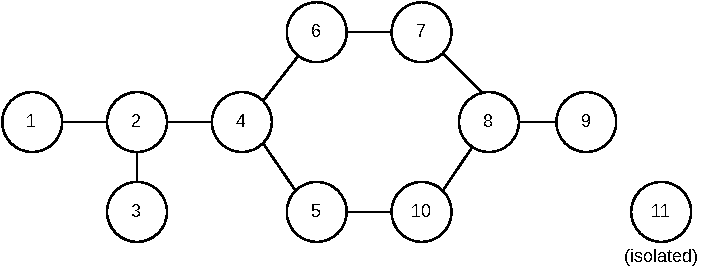
\includegraphics[width=0.9\textwidth]{./img/ex-greedy.pdf}%
    \caption{A sample graph $G$.}\label{fig:ex-greedy}%
\end{figure}

\begin{table}[htbp]
\caption{\label{tab:greedy}Deriving variable order for the BDD encoding UFLP, for the graph depicted in Figure \ref{fig:ex-greedy}. Highlighted are changes as compared to the previous number.}
\centering
\begin{tabular}{rllrrllll}
\textcircled{$i$} & \(S_i\) & \(S^*_i\) & \(\vert S^*_i\vert\) & \(k=1\) & \(k=5\) & \(k=8\) & \(k=11\) & \(k=12\)\\
\hline
1 & \{1,2\} & \{1,2,3,4\} & 4 & 4 & \hl{X} & X & X & X\\
2 & \{1,2,3\} & \{1,2,3,4,5,6\} & 6 & 6 & \hl{2} & \hl{X} & X & X\\
3 & \{2,3\} & \{1,2,3,4\} & 4 & 4 & \hl{X} & X & X & X\\
4 & \{2,4,5,6\} & \{1,2,3,4,5,6,7,10\} & 8 & 8 & \hl{4} & \hl{2} & \hl{X} & X\\
5 & \{4,5,10\} & \{2,4,5,6,8,10\} & 6 & 6 & \hl{4} & \hl{2} & \hl{1} & \hl{X}\\
6 & \{4,6,7\} & \{2,4,5,6,7,8\} & 6 & 6 & \hl{4} & \hl{2} & \hl{1} & \hl{X}\\
7 & \{6,7,8\} & \{4,6,7,8,9,10\} & 6 & 6 & \hl{5} & \hl{4} & \hl{2} & \hl{1}\\
8 & \{7,8,9,10\} & \{5,6,7,8,9,10\} & 6 & 6 & 6 & \hl{4} & \hl{2} & \hl{1}\\
9 & \{8,9\} & \{7,8,9,10\} & 4 & 4 & 4 & 4 & \hl{2} & \hl{1}\\
10 & \{5, 8, 10\} & \{4,5,7,8,9,10\} & 6 & 6 & \hl{5} & \hl{4} & \hl{2} & \hl{1}\\
11 & \{11\} & \{11\} & 1 & \hl{X} & X & X & X & X\\
 &  &  &  &  &  &  &  & \\
\end{tabular}
\end{table}

\end{example}

In practice, the presented algorithm provides relatively compact BDD sizes.
\marginnote{In fact, I am almost sure the algorihtm is optimal. Proof sketch: use
Proposition \ref{prop:bestDD} to construct a better order. Note that an order
is a sequence of subsets corresponding to distance-2-neighborhoods. Pick the first
pair of adjacent subsets in the solution such that a greedy algorithm would invert their order,
and swap them. I think that looking at a picture similar to Figures \ref{fig:LW-ex} one can show
that such swap would never make the resulting BDD size worse. Hence, ``fixing'' all such
discrepancies we arrive at a solution that can be obtained with the greedy algorithm.}[-15em]
\section{Creating a j-UFLP instance.}
\label{sec:org0a6dbae}

\section{A numerical experiment}
\label{sec:orgaf624d5}

\printbibliography
\end{document}